%-----------------------------------------------------------------------------
\chapter{\babEmpat}
%-----------------------------------------------------------------------------

The 46 supervised models and four vision-language zero-shot endpoints are scored on the same 104-image held-out test set across three comparative axes: classification performance, inference latency, and operational cost. Macro F1 is the primary performance metric and Mature Recall is the secondary metric, both reported with 1000-resample bootstrap 95\% confidence intervals computed under paired indices so cross-track comparisons remain on the same draws.


% =============================================================
\section{Cross-Validation Results}

Five-fold stratified cross-validation over 1036 images scores every classical machine learning configuration, every deep learning backbone, and every hybrid configuration on Macro F1 with the same class-balanced fold assignment. The per-track results below isolate within-family behavior before pooling for the cross-track ranking.

\subsection{Classical Machine Learning}

The 40-configuration sweep across five algorithms (Random Forest, Support Vector Machine with radial basis kernel, K-Nearest Neighbors, Logistic Regression, Gradient Boosting) and eight color vegetation indices identifies Support Vector Machine with radial basis kernel as the dominant classical algorithm under cross-validation. All three leading configurations select the ExGR (Excess Green minus Excess Red) vegetation index, with the Support Vector Machine, Gradient Boosting, and Random Forest classifiers occupying the top three slots respectively. The complete ranking of all 40 configurations is reported in Appendix A.

\begin{table}[H]
    \centering
    \caption{Top 3 Classical ML Configurations (CV)}
    \label{tab:cv-ml-top3}
    \begin{tabular}{clll}
        \hline
        Rank & Vegetation index & Algorithm & CV Macro F1 $\pm$ Std \\
        \hline
        1 & ExGR & SVM (RBF) & $0.9502 \pm 0.0070$ \\
        2 & ExGR & Gradient Boosting & $0.9465 \pm 0.0139$ \\
        3 & ExGR & Random Forest & $0.9418 \pm 0.0141$ \\
        \hline
    \end{tabular}
\end{table}

\subsection{Deep Learning}

The three lightweight backbones fine-tuned under two-phase transfer learning produce a clear cross-validation ordering: EfficientNetB0 leads with the lowest fold-to-fold variance, MobileNetV2 sits in the middle at roughly four percentage points behind, and MobileNetV3-Small trails at the bottom. The compound-scaling backbone benefits the most from limited supervision over canopy-level RGB. The cross-validation ordering does not carry to the held-out split between the two MobileNet variants: MobileNetV3-Small recovers above MobileNetV2 on the test set, while EfficientNetB0 retains its lead.

\begin{table}[H]
    \centering
    \caption{Deep Learning Backbones (CV)}
    \label{tab:cv-dl}
    \begin{tabular}{ll}
        \hline
        Backbone & CV Macro F1 $\pm$ Std \\
        \hline
        EfficientNetB0      & $0.9664 \pm 0.0086$ \\
        MobileNetV2         & $0.9270 \pm 0.0170$ \\
        MobileNetV3-Small   & $0.9083 \pm 0.0143$ \\
        \hline
    \end{tabular}
\end{table}

\subsection{Hybrid}

The late-fusion hybrid concatenates the 1280-dimensional EfficientNetB0 embedding with the 18-dimensional handcrafted descriptor per vegetation index, sweeping NGRDI, ExGR, and VARI as the handcrafted source. NGRDI takes the top cross-validation Macro F1 across all 46 supervised models, with the three hybrid configurations all surpassing the strongest deep learning backbone.

\begin{table}[H]
    \centering
    \caption{Hybrid Configurations (CV)}
    \label{tab:cv-hybrid}
    \begin{tabular}{ll}
        \hline
        Vegetation index & CV Macro F1 $\pm$ Std \\
        \hline
        NGRDI & $\mathbf{0.9770 \pm 0.0092}$ \\
        ExGR  & $0.9691 \pm 0.0089$ \\
        VARI  & $0.9541 \pm 0.0174$ \\
        \hline
    \end{tabular}
\end{table}

\subsection{Cross-Track Summary}

The cross-validation ordering across the three supervised families is Hybrid above Deep Learning above Classical Machine Learning, with the best Hybrid (NGRDI, $0.9770$) leading the best Deep Learning (EfficientNetB0, $0.9664$) by about $1.1$ percentage points and the best Classical (ExGR plus Support Vector Machine, $0.9502$) by about $2.7$ percentage points. The dispersion across folds is tightest in the Deep Learning track (Std $0.0086$ for EfficientNetB0) and the Hybrid track (Std $0.0089$--$0.0092$), suggesting that the fold-to-fold instability seen in the Classical track (Std up to $0.0197$ at Random Forest with RGBVI) reflects sensitivity of low-dimensional kernels and tree ensembles to which images land in the validation fold.

% =============================================================
% PANDUAN GAMBAR MANUAL UNTUK GAMBAR 4.1.4 — CV ranking bar across 46 supervised models
% Tujuan: visualisasi sekali pandang yang menempatkan 40 ML + 3 DL + 3 Hybrid pada satu sumbu.
% Susunan: horizontal bar chart, 46 baris, sorted descending by mean Macro F1; error bar = Std across 5 folds.
% Warna per track: ML biru, DL hijau, Hybrid merah; legend di pojok bawah.
% Cara generate (di notebook ml/Thesis_DL_Compare_3Class):
%   1. Kumpulkan dict {model_name: (mean_f1, std_f1, track)} dari ketiga sumber notebook.
%   2. plt.barh(y, mean, xerr=std, color=track_color).
%   3. ylim sorted, xlim 0.85--1.00.
%   4. plt.savefig('img/Fig 4.1.4 CV Ranking 46 Models.png', dpi=200, bbox_inches='tight').
% Simpan sebagai: img/Fig 4.1.4 CV Ranking 46 Models.png
% =============================================================
\begin{figure}[H]
    \centering
    \includegraphics[width=\textwidth]{img/Fig 4.1.4 CV Ranking 46 Models.png}
    \caption{CV Ranking, 46 Supervised Models}
    \label{fig:cv-ranking}
\end{figure}


% =============================================================
\section{Test Set Results}

After cross-validation each configuration is refit on the full 1036-image pool and evaluated once on the 104-image held-out test set, with class support 49 Vegetative, 34 Generative, and 21 Mature. Bootstrap 95\% confidence intervals are computed under 1000 paired resampling draws shared across the 46 supervised models and the four evaluated vision-language endpoints so cross-model comparisons remain on the same sample.

\subsection{Supervised Pool}

The supervised test ranking moves the Hybrid winner from NGRDI to ExGR, leaves the EfficientNetB0 backbone in the Deep Learning lead, and keeps Support Vector Machine plus ExGR as the strongest Classical configuration. Point estimates compress into a narrow band between Macro F1 $0.94$ and $0.97$ for the top of each family.

\begin{table}[H]
    \centering
    \caption{Supervised Configurations on Test Set (Sorted by Macro F1)}
    \label{tab:test-top}
    \footnotesize
    \setlength{\tabcolsep}{4pt}
    \renewcommand{\arraystretch}{1.15}
    \begin{tabular}{@{}llcc@{}}
        \hline
        Track & Configuration & Test Macro F1 [95\% CI] & Mature Recall [95\% CI] \\
        \hline
        Hybrid & EfficientNetB0 + ExGR  & $0.9662$ [$0.9215$, $1.0000$] & $0.9553$ [$0.8398$, $1.0000$] \\
        Hybrid & EfficientNetB0 + NGRDI & $0.9621$ [$0.9133$, $1.0000$] & $0.9553$ [$0.8398$, $1.0000$] \\
        ML     & SVM (RBF) + ExGR       & $0.9577$ [$0.9106$, $0.9916$] & $0.9507$ [$0.8500$, $1.0000$] \\
        DL     & EfficientNetB0         & $0.9532$ [$0.8998$, $0.9921$] & $0.9068$ [$0.7619$, $1.0000$] \\
        Hybrid & EfficientNetB0 + VARI  & $0.9454$ [$0.8898$, $0.9912$] & $0.9553$ [$0.8398$, $1.0000$] \\
        ML     & RandomForest + ExGR    & $0.9368$ [$0.8831$, $0.9811$] & $0.9030$ [$0.7647$, $1.0000$] \\
        DL     & MobileNetV3-Small      & $0.9198$ [$0.8497$, $0.9732$] & $0.8591$ [$0.6874$, $1.0000$] \\
        DL     & MobileNetV2            & $0.8821$ [$0.8081$, $0.9440$] & $0.7656$ [$0.5625$, $0.9444$] \\
        \hline
    \end{tabular}
\end{table}

% Bootstrap CI diisi dari img/bootstrap_ci_test.csv (1000 paired resamples, percentile [2.5, 97.5]).

\subsection{Vision-Language Zero-Shot}

Four hosted endpoints (Gemini 2.5 Flash, Gemini 2.5 Flash Lite, GPT-4o, GPT-4o mini) are exercised under a single structured prompt with temperature 0 and the internal reasoning step disabled where the API exposes that option, and evaluated on the identical 104-image test set without any rice-specific fine-tuning. Per-call output is parsed as JSON with the classification, the confidence score, and the gatekeeper accept flag, so models that decline a frame as out-of-distribution are recorded as rejects rather than as misclassifications.

\begin{table}[H]
    \centering
    \caption{VLM Zero-Shot Results (Test)}
    \label{tab:test-vlm}
    \footnotesize
    \setlength{\tabcolsep}{4pt}
    \renewcommand{\arraystretch}{1.15}
    \begin{tabular}{@{}lcccc@{}}
        \hline
        Model & Accept & Test Macro F1 [95\% CI] & Mature Recall [95\% CI] & Acc. \\
        \hline
        Gemini 2.5 Flash Lite & $0.952$ & $\mathbf{0.941}$ [$0.9126$, $0.9909$] & $1.000$ [$1.000$, $1.000$] & $0.949$ \\
        GPT-4o mini           & $1.000$ & $0.892$ [$0.8649$, $0.9637$]          & $0.952$ [$0.9268$, $1.000$] & $0.913$ \\
        GPT-4o                & $0.990$ & $0.831$ [$0.8170$, $0.9349$]          & $1.000$ [$1.000$, $1.000$] & $0.864$ \\
        Gemini 2.5 Flash      & $1.000$ & $0.811$ [$0.7950$, $0.9180$]          & $1.000$ [$1.000$, $1.000$] & $0.846$ \\
        \hline
    \end{tabular}
\end{table}

The strongest zero-shot endpoint is Gemini 2.5 Flash Lite at Macro F1 $0.941$, which sits $0.025$ Macro F1 below the supervised Hybrid leader at $0.9662$ and $0.017$ below the Classical leader at $0.9577$. The smaller-than-expected gap is shaped by a class-specific failure pattern: all four endpoints over-trigger the Mature label on Generative frames at varying severity (Gemini Flash $14/34$, GPT-4o $13/34$, GPT-4o mini $7/34$, Flash Lite $3/31$ on accepted Generative frames), so Macro F1 is dragged down by Generative recall while Mature Recall stays at $0.952$ or above on accepted samples. The pattern is vendor-agnostic, scales inversely with model size, and is consistent with a prompt-bound interpretation of mature canopy cues. The gatekeeper-style rejection behavior on rice imagery itself splits across endpoints: Flash Lite rejects five frames (one Vegetative, three Generative, one Mature) for a $4.81\%$ false-reject rate, GPT-4o rejects a single sparse early-stage Vegetative frame ($0.96\%$ false-reject rate), and Flash and GPT-4o mini reject none.

\subsection{CI Overlap}

The point-estimate gap between the strongest Hybrid (ExGR, $0.9662$) and the strongest Classical configuration (Support Vector Machine plus ExGR, $0.9577$) is $0.0085$ on Macro F1, which is roughly an order of magnitude smaller than the bootstrap 95\% interval width on the Classical configuration ($0.0810$). The bootstrap intervals on Macro F1 of the top eight configurations all overlap, so the cross-track ordering Hybrid above Classical above Deep Learning is not statistically distinguishable on the held-out sample, and the comparative conclusion has to rest on the joint Pareto view together with the operational-cost axis.

% Fig 4.2.3 sudah di-generate dari ml/Bab4_Figures.ipynb (load bootstrap_ci_test.csv).
\begin{figure}[H]
    \centering
    \includegraphics[width=0.85\textwidth]{img/Fig 4.2.3 Bootstrap CI Forest.png}
    \caption{Bootstrap 95\% CI Forest Plot}
    \label{fig:ci-forest}
\end{figure}


% =============================================================
\section{Cross-Track Ranking}

The 50 evaluated models (46 supervised plus four vision-language endpoints) are aggregated under a single ranking, first against Macro F1 alone, then against Mature Recall alone, then jointly on the Pareto frontier of the two metrics. The two single-metric rankings disagree on which configurations occupy the top slots, and the joint Pareto view is reported alongside because the IoT-critical concern that Mature timing is reported correctly cannot be reduced to the primary metric.

\subsection{Macro F1 Ranking}

The top five on Macro F1 are dominated by Hybrid (three of five), followed by the strongest Classical configuration and the strongest Deep Learning backbone. The ranking is compact: the gap from rank 1 to rank 5 is $0.0208$ Macro F1, smaller than the width of the bootstrap interval reported above for the Classical leader.

\begin{table}[H]
    \centering
    \caption{Top 5 by Macro F1 (Test)}
    \label{tab:rank-f1}
    \begin{tabular}{cllll}
        \hline
        Rank & Track & Configuration & Test Macro F1 & Mature Recall \\
        \hline
        1 & Hybrid & EfficientNetB0 + ExGR  & $0.9662$ & $0.9553$ \\
        2 & Hybrid & EfficientNetB0 + NGRDI & $0.9621$ & $0.9553$ \\
        3 & ML     & SVM (RBF) + ExGR       & $0.9577$ & $0.9507$ \\
        4 & DL     & EfficientNetB0         & $0.9532$ & $0.9068$ \\
        5 & Hybrid & EfficientNetB0 + VARI  & $0.9454$ & $0.9553$ \\
        \hline
    \end{tabular}
\end{table}

\subsection{Mature Recall Ranking}

Ranking by Mature Recall alone surfaces a different leader board: three Classical configurations sit at the top, all using green-minus-red vegetation indices with Gradient Boosting or Logistic Regression heads. The top entries by Mature Recall do not appear in the top five by Macro F1, which is the trade-off the joint metric protocol is designed to make visible.

\begin{table}[H]
    \centering
    \caption{Top 3 by Mature Recall (Test)}
    \label{tab:rank-mature}
    \footnotesize
    \setlength{\tabcolsep}{5pt}
    \renewcommand{\arraystretch}{1.15}
    \begin{tabular}{@{}clcccc@{}}
        \hline
        Rank & Track & Configuration & Mature Recall & CV Macro F1 & Test Macro F1 \\
        \hline
        1 & ML & GradBoost + NGRDI & $1.0000$ & $0.9375$ & $0.9099$ \\
        2 & ML & GradBoost + MGRVI & $1.0000$ & $0.9290$ & $0.9020$ \\
        3 & ML & LogReg + VARI     & $1.0000$ & $0.8938$ & $0.8766$ \\
        \hline
    \end{tabular}
\end{table}

\subsection{Joint Pareto}

The Pareto frontier on the two metrics contains the Hybrid configurations (high Macro F1 with Mature Recall $0.9553$), the Classical leader Support Vector Machine plus ExGR (Macro F1 $0.9577$ with Mature Recall $0.9507$), and the Mature-specialist Classical configurations that trade Macro F1 for the highest Mature Recall. Models inside the frontier are dominated on both metrics and are not considered for deployment selection.

% =============================================================
% PANDUAN GAMBAR MANUAL UNTUK GAMBAR 4.3.3 — Pareto scatter
% Tujuan: visualisasi trade-off Macro F1 vs Mature Recall, dengan Pareto frontier ditandai.
% Susunan: scatter 50 titik (40 ML + 3 DL + 3 Hybrid + 4 VLM), Pareto frontier connected line, color per track.
% Cara generate:
%   1. Load semua hasil test (macro_f1, mature_recall) per model.
%   2. Compute Pareto frontier (no model dominates both).
%   3. plt.scatter per track; plt.plot(pareto_x, pareto_y, 'k--') untuk frontier.
%   4. Annotate top 3 di frontier dengan nama config.
%   5. plt.savefig('img/Fig 4.3.3 Pareto Macro F1 vs Mature Recall.png', dpi=200, bbox_inches='tight').
% Simpan sebagai: img/Fig 4.3.3 Pareto Macro F1 vs Mature Recall.png
% =============================================================
\begin{figure}[H]
    \centering
    \includegraphics[width=0.85\textwidth]{img/Fig 4.3.3 Pareto Macro F1 vs Mature Recall.png}
    \caption{Pareto: Macro F1 vs Mature Recall}
    \label{fig:pareto-joint}
\end{figure}


% =============================================================
\section{Per-Class Diagnostics}

The aggregated rankings hide where each track makes mistakes. The confusion structure on the held-out set isolates which class pairs are confused and the permutation-importance scan on the Classical leader identifies which handcrafted features drive the Support Vector Machine boundary.

\subsection{Confusion Matrix}

The Classical leader (Support Vector Machine plus ExGR) misclassifies 4 of 104 test images and produces per-class precision-recall-F1 of $0.98$/$0.96$/$0.97$ on Vegetative, $0.94$/$0.97$/$0.96$ on Generative, and $0.95$/$0.95$/$0.95$ on Mature. The Vegetative-Generative pair carries the most residual confusion, consistent with the canopy color overlap during stem elongation and panicle initiation; the Mature class is misclassified less in aggregate but each error costs more under the harvest-timing objective.

% =============================================================
% PANDUAN GAMBAR MANUAL UNTUK GAMBAR 4.4.1 — Confusion matrix grid
% Tujuan: visualisasi pola misklasifikasi per track pada test set yang sama.
% Susunan: 2x2 grid heatmap (3x3 confusion matrix per panel) untuk:
%   (a) ML: SVM (RBF) + ExGR
%   (b) DL: EfficientNetB0
%   (c) Hybrid: EfficientNetB0 + ExGR
%   (d) VLM: Gemini 2.5 Flash Lite (top VLM by Macro F1)
% Cara generate:
%   1. Load y_true, y_pred per model dari notebook.
%   2. sklearn.metrics.confusion_matrix(y_true, y_pred, labels=['Vegetative','Generative','Mature']).
%   3. seaborn.heatmap(cm, annot=True, fmt='d', cmap='Blues') per subplot.
%   4. plt.savefig('img/Fig 4.4.1 Confusion Matrix Grid.png', dpi=200, bbox_inches='tight').
% Simpan sebagai: img/Fig 4.4.1 Confusion Matrix Grid.png
% =============================================================
\begin{figure}[H]
    \centering
    \includegraphics[width=\textwidth]{img/Fig 4.4.1 Confusion Matrix Grid.png}
    \caption{Confusion Matrices, Top per Track}
    \label{fig:confusion-grid}
\end{figure}

\subsection{Feature Importance}

Permutation importance computed with 30 repeats on the Classical leader (Support Vector Machine plus ExGR) ranks the dispersion of the ExGR signal as the dominant feature, with a magnitude roughly four times larger than the second-ranked feature. The top five comprise two ExGR statistics and three Gray Level Co-occurrence Matrix descriptors, which confirms that the boundary is supported by the joint chromatic-plus-texture descriptor rather than by a single dominant statistic.

\begin{table}[H]
    \centering
    \caption{Top 5 Permutation-Importance Features}
    \label{tab:feature-importance}
    \begin{tabular}{cll}
        \hline
        Rank & Feature & Importance $\pm$ Std \\
        \hline
        1 & ExGR\_std            & $0.1408 \pm 0.0380$ \\
        2 & glcm\_energy\_mean   & $0.0312 \pm 0.0187$ \\
        3 & ExGR\_p10            & $0.0301 \pm 0.0155$ \\
        4 & glcm\_homogeneity\_std & $0.0287 \pm 0.0204$ \\
        5 & glcm\_contrast\_std  & $0.0259 \pm 0.0096$ \\
        \hline
    \end{tabular}
\end{table}

\begin{figure}[H]
    \centering
    \includegraphics[width=0.8\textwidth]{img/Fig 4.4.2 Feature Importance.png}
    \caption{Permutation Importance, 18 Handcrafted Features}
    \label{fig:feature-importance}
\end{figure}


% =============================================================
\section{Field Validation}

The bench-scale rig (four polybag-grown plants inside a single litter box with the ESP32-CAM mounted overhead at fixed height) is exercised across three scenarios: end-to-end capture-cycle latency, gatekeeper behavior on non-rice probes, and Mature carry-over measured against the curated test-set Mature Recall. The polybag plants are at the Mature stage for the full duration of the validation, so the rice-class measurements are reported for Mature only.

\subsection{Latency}

End-to-end latency is recorded per capture as the round-trip time between the ESP32-CAM HTTP trigger and the response return, instrumented at four checkpoints: device-side trigger ($T_1$), server-side receive ($T_2$), inference-done ($T_3$), and response-ready ($T_4$). The deployed pipeline runs the Gemini 2.5 Flash Lite gatekeeper followed by the Hybrid CNN classifier on a single Cloud Run service in asia-southeast2 with 1 vCPU and 512 MiB of memory. The ESP32-CAM captures at QXGA resolution (around 200 KB per JPEG) and posts directly to the inference endpoint, which gives a clean separation between transport and compute.

\begin{table}[H]
    \centering
    \caption{End-to-End Capture Cycle Latency}
    \label{tab:field-latency}
    \begin{tabular}{lrrr}
        \hline
        Stage & $n$ & Median (ms) & p95 (ms) \\
        \hline
        End-to-end (ESP $T_1 \to T_{resp}$)                 & $12$ & $8570$ & $29878$ \\
        \quad Network and upload (HTTP+TLS+payload)         & $12$ & $3688$ & $10901$ \\
        Server total ($T_2 \to T_4$)                        & $51$ & $4006$ & $7750$ \\
        \quad JPEG decode                                   & $51$ & $23$   & $36$ \\
        \quad Gatekeeper LLM and CNN compute                & $51$ & $3865$ & $7592$ \\
        \quad Response wrap                                 & $36$ & $128$  & $164$ \\
        \hline
        Path: gatekeeper rejected (LLM only)                & $15$ & $4692$ & $6488$ \\
        Path: accepted (LLM and Hybrid CNN)                 & $36$ & $3868$ & $9284$ \\
        \hline
    \end{tabular}
\end{table}

\begin{figure}[H]
    \centering
    \includegraphics[width=0.85\textwidth]{img/Fig 4.5.1 Latency Distribution.png}
    \caption{Cloud Run server-side latency distribution, accepted vs rejected paths}
    \label{fig:latency-distribution}
\end{figure}

Server-side compute is dominated by the gatekeeper. JPEG decode at $23$ ms is negligible. The bulk of the server-side budget, $3865$ ms median, comes from the remote Gemini 2.5 Flash Lite API call, since the gatekeeper is invoked on every request before the local Hybrid CNN runs.

The accepted-path median ($3868$ ms) is lower than the rejected-path median ($4692$ ms), which inverts the naive expectation that the path running both tiers must be slower. The pattern is consistent across the run: clear rice frames trigger a short gatekeeper response (terse accept reasoning, fewer output tokens), while ambiguous frames generate longer rejection reasoning that explains why the image is not usable. Tier-2 CNN inference on the accepted path is fast enough that it cannot offset the gatekeeper reasoning gap.

Network plus upload, measured on the ESP32-CAM side, contributes $3688$ ms median. The figure includes WiFi upload of a $200$ KB QXGA JPEG, TLS handshake, and Cloud Run routing, not just packet transit. End-to-end median of $8.57$ s is dominated by these two stages in roughly equal proportion. The end-to-end p95 of $29.88$ s is driven by a single cold-start outlier on the first request after Cloud Run scale-from-zero with model load, with the corresponding server-side latency for that outlier reaching $37.97$ s. Excluding the cold start, server-side p95 stays at $7.75$ s. The pipeline is acceptable for the deployment cadence of one capture cycle every ten minutes, well below the cycle period.

\subsection{Non-Rice Gatekeeper}

The gatekeeper is probed with twelve non-rice frames (four empty-litter-box frames, four with a hand in the field of view, four with a non-rice plant) routed through each of the four vision-language endpoints. The reject rate per endpoint and the stated reason from the prompt response together characterize whether the open-world rejection is reliable enough for deployment.

\begin{table}[H]
    \centering
    \caption{Gatekeeper Reject Behavior (Non-Rice Probe)}
    \label{tab:field-gatekeeper}
    \begin{tabular}{lrr}
        \hline
        Endpoint & Reject (of 12) & Reject rate \\
        \hline
        Gemini 2.5 Flash       & $12$ & $100\%$ \\
        Gemini 2.5 Flash Lite  & $12$ & $100\%$ \\
        GPT-4o                 & $12$ & $100\%$ \\
        GPT-4o mini            & $12$ & $100\%$ \\
        \hline
    \end{tabular}
\end{table}

The false-accept rate on the non-rice probe is zero across all four endpoints. The false-reject rate on the curated rice test set varies by endpoint: Gemini 2.5 Flash Lite rejects $5/104 = 4.81\%$ (one Vegetative, three Generative, one Mature), GPT-4o rejects $1/104 = 0.96\%$ (one sparse early-vegetative frame), and Gemini 2.5 Flash and GPT-4o mini reject zero. The deployed pipeline uses Gemini 2.5 Flash Lite, so the operational gatekeeper envelope is a $4.81\%$ false-reject rate on rice imagery against a $0\%$ false-accept rate on non-rice probes, which is the empirical regime that supports the open-set rejector role assigned to the vision-language gatekeeper.

\begin{figure}[H]
    \centering
    \includegraphics[width=0.85\textwidth]{img/Fig 4.5.2 Gatekeeper.png}
    \caption{Gatekeeper FRR and FAR}
    \label{fig:gatekeeper-bars}
\end{figure}

\subsection{Mature on ESP32-CAM}

Fifty-one ESP32-CAM Mature captures from the bench-scale rig are routed through both supervised leaders and the four-model vision-language cohort, and Mature Recall on this subset is compared in paired form to Mature Recall on the curated test subset. Any degradation attributable to the ESP32-CAM sensor (color rendering, lens geometry, JPEG compression at the device) and to the controlled indoor lighting of the rig becomes visible as a per-class delta in the same metric used to rank the supervised pool.

\begin{table}[H]
    \centering
    \caption{Mature Recall: Curated Test vs ESP32-CAM Bench}
    \label{tab:field-mature-carry}
    \footnotesize
    \setlength{\tabcolsep}{5pt}
    \renewcommand{\arraystretch}{1.15}
    \begin{tabular}{@{}llccc@{}}
        \hline
        Classifier & Track & Curated ($n{=}21$) & Bench ($n{=}51$) & $\Delta$ (pp) \\
        \hline
        Hybrid + ExGR          & Supervised & $0.9553$ & $\mathbf{1.0000}$ & $+4.5$  \\
        SVM (RBF) + ExGR       & Supervised & $0.9507$ & $0.0000$          & $-95.1$ \\
        GPT-4o                 & VLM        & $1.0000$ & $\mathbf{1.0000}$ & $0.0$   \\
        Gemini 2.5 Flash       & VLM        & $1.0000$ & $0.8824$          & $-11.8$ \\
        Gemini 2.5 Flash Lite  & VLM        & $0.9524$ & $0.8824$          & $-7.0$  \\
        GPT-4o mini            & VLM        & $0.9524$ & $0.4118$          & $-54.1$ \\
        \hline
    \end{tabular}
\end{table}

Mature Recall in this table is computed with the full true-Mature count as the denominator on both partitions, so a rejection by the vision-language gatekeeper counts as a miss against recall. The two supervised leaders diverge sharply on ESP32-CAM imagery. The Hybrid configuration improves by $4.5$ percentage points to perfect Mature Recall, while the Classical configuration collapses by $95.1$ percentage points to $0.0000$: every one of the $51$ bench frames is misclassified, $47$ as Vegetative and $4$ as Generative. The handcrafted descriptor is computed over the full unmasked frame rather than a canopy-only crop, so it mixes background and lighting statistics into the same 18-dimensional vector on which the classifier was fit. The curated training images are cropped tight to the canopy; the ESP32-CAM bench frames carry more background (litter box, soil, adjacent polybags) at a fixed overhead distance, which shifts the ExGR and GLCM statistics of a genuinely Mature frame closer to the region of feature space the classifier associates with sparse, early-stage Vegetative canopy. The Hybrid configuration is not exposed to this failure mode because its convolutional branch reads the raw image directly and is not limited to the 18-dimensional descriptor. A branch-ablation check narrows down where the robustness comes from. Feeding the Hybrid fusion head the real 18-dimensional descriptor with the image branch replaced by a neutral gray frame still classifies all $51$ bench frames as Mature, at $0.84$--$0.91$ confidence; feeding it the real image with the descriptor branch zeroed out does the same, at confidence levels matching the full model. The same 18 numbers that the Classical SVM reads as Vegetative are read correctly by the Hybrid fusion head, so the descriptor itself is not the point of failure; the SVM's RBF decision boundary is. A radial-basis kernel is a local method, its prediction for a point far from any training example is driven by whichever training cluster happens to be nearest in feature space, which for these bench frames is Vegetative. The fusion head's decision surface over the same descriptor was shaped jointly with the image branch during training and does not collapse to the nearest training cluster in the same way. This result is the strongest evidence in the comparative study for preferring the Hybrid classifier at deployment: the two configurations are statistically indistinguishable on the curated test set ($0.9662$ vs.\ $0.9577$ Macro F1), but only one of them keeps working once the sensor changes. The vision-language cohort splits sharply as well. GPT-4o retains perfect Mature Recall on bench imagery, Gemini 2.5 Flash loses $11.8$ percentage points by classifying six bench frames as out-of-distribution, Gemini 2.5 Flash Lite loses $7.0$ percentage points (one curated Mature rejected plus six bench frames rejected for a representative reason returned by the endpoint that the frame shows ``harvested or dried rice material, not a standing rice canopy in a field''), and GPT-4o mini collapses by $54.1$ percentage points by rejecting $30$ of $51$ bench frames on the same domain mismatch. The drop does not scale monotonically with model capacity: GPT-4o, the largest endpoint tested, retains perfect Mature Recall on bench imagery, while GPT-4o mini, the smallest, collapses by $54.1$ percentage points despite sharing the same provider's pretraining regime. The asymmetry suggests that the smaller endpoint applies a narrower field-rice template in which polybag-grown mature rice under indoor ambient light does not qualify as a standing rice canopy, a prior that the larger model overrides with sufficient visual context to recognize the class correctly. The drop within the Gemini family is more moderate and follows capacity order, which is consistent with a field-imagery prior that becomes a harder constraint as model size decreases.

\begin{figure}[H]
    \centering
    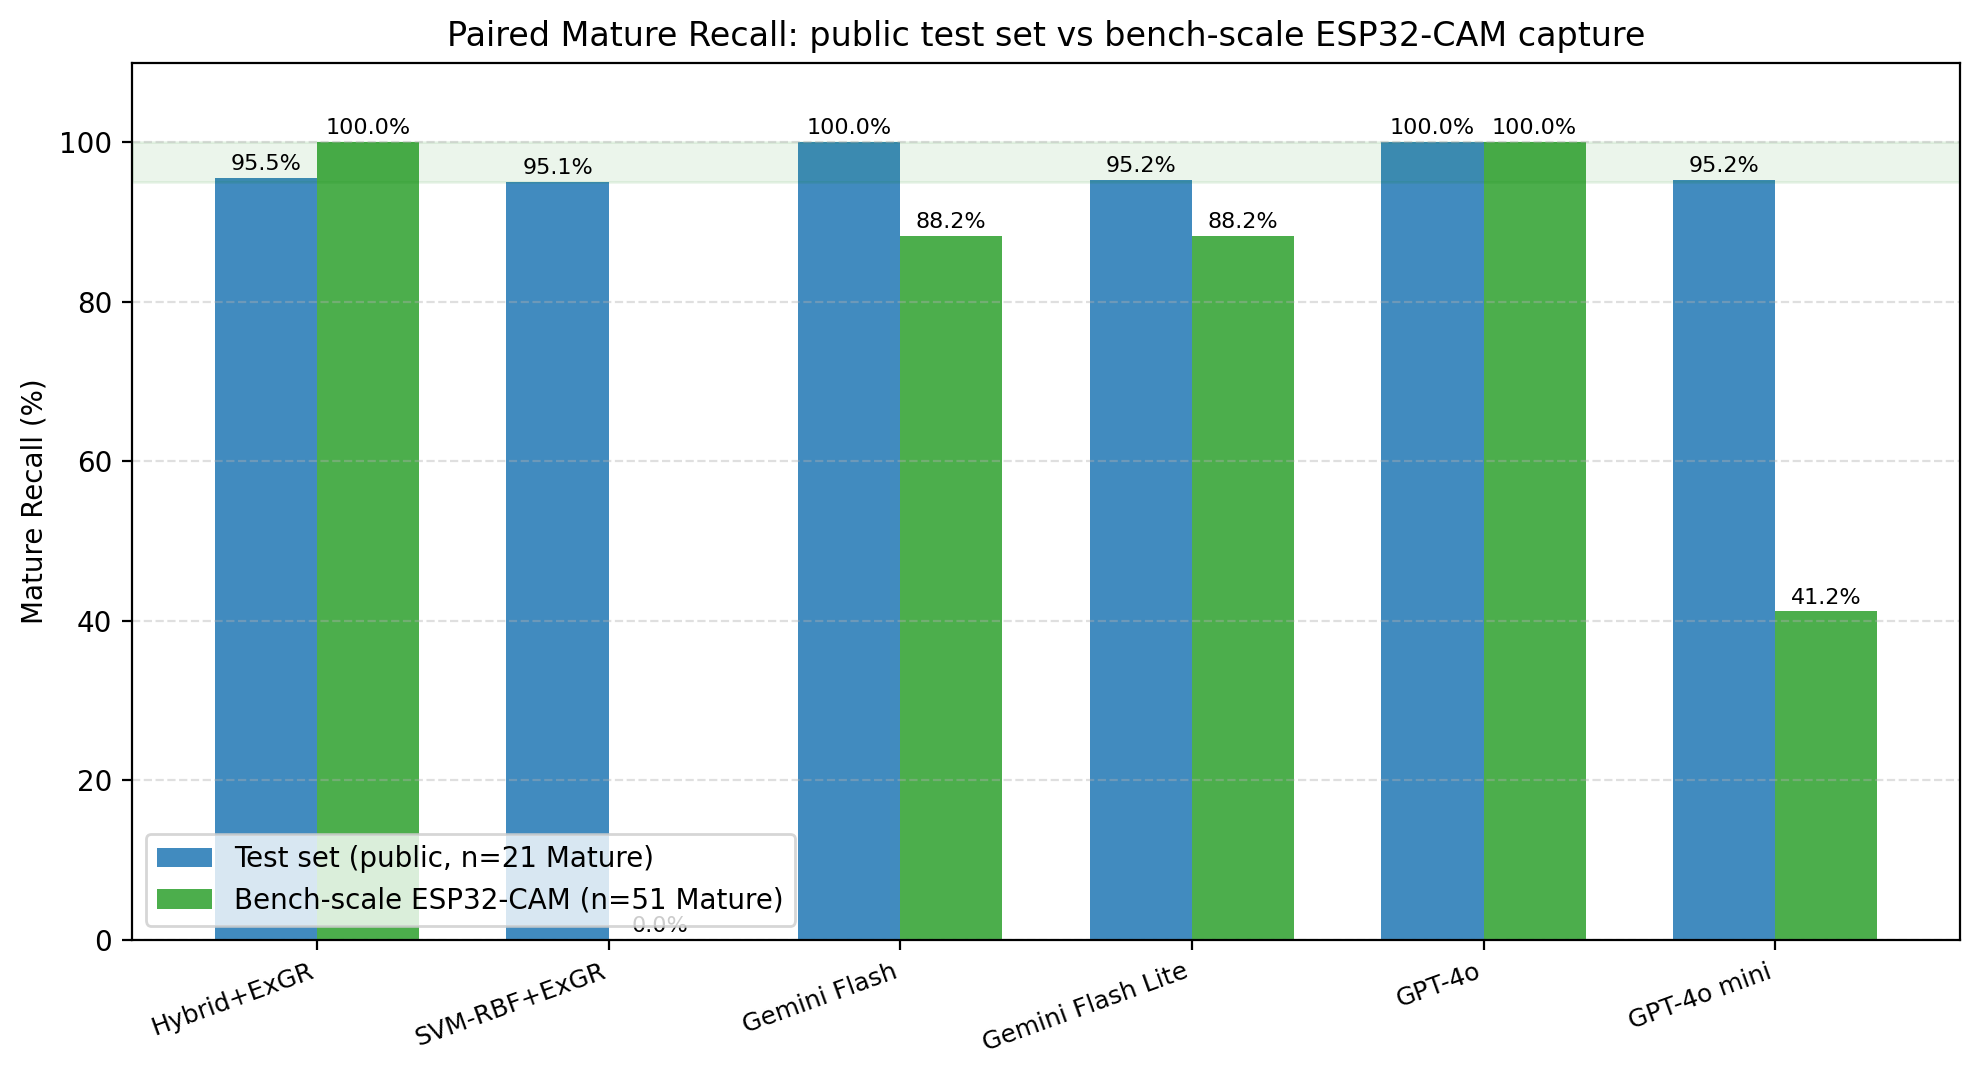
\includegraphics[width=0.85\textwidth]{img/Fig 4.5.3 Domain Shift.png}
    \caption{Mature Recall Delta: Curated vs ESP32-CAM Bench}
    \label{fig:domain-shift}
\end{figure}

\begin{figure}[H]
    \centering
    \includegraphics[width=0.85\textwidth]{img/Fig 4.5.3 VLM Rejections.png}
    \caption{ESP32-CAM Frames Rejected by GPT-4o Mini}
    \label{fig:vlm-rejections}
\end{figure}


% =============================================================
\section{Operational Cost}

The third comparative axis is operational cost, which decomposes into model artifact footprint, per-inference Cloud Run compute, and per-call vision-language API price. The Classical leader serializes to a $55$ KB joblib file, more than two orders of magnitude smaller than the $\sim$$17$ MB EfficientNetB0 SavedModel that backs both the Deep Learning leader and the Hybrid leader, and the footprint difference compounds at Cloud Run cold start because the tiny artifact loads on the first request without a perceptible delay while the EfficientNetB0 SavedModel measurably extends the wall-clock time that Cloud Run bills for. Cloud Run second-generation pricing in the Jakarta region charges per vCPU-second, per GiB-second of memory, and a fixed per-request component on a 1 vCPU and 512 MiB revision. The vision-language endpoints add a per-call billing layer that spans about $25$-fold within the vision-language cohort between Gemini 2.5 Flash Lite at $\sim$\$$0.045$ per thousand calls and GPT-4o at $\sim$\$$1.13$ per thousand calls under the structured prompt of about 250 input tokens and 50 output tokens, and more than two orders of magnitude relative to the Classical inference path.

\begin{table}[H]
    \centering
    \caption{Operational Cost Summary}
    \label{tab:cost-summary}
    \footnotesize
    \setlength{\tabcolsep}{4pt}
    \renewcommand{\arraystretch}{1.15}
    \begin{tabular}{@{}p{55mm}cp{45mm}r@{}}
        \hline
        Track / Endpoint & Artifact & Inference path & USD / 1k \\
        \hline
        Classical: SVM (RBF) + ExGR    & $55$ KB        & 18-dim $\rightarrow$ RBF kernel        & $\sim 0.003$  \\
        DL: EfficientNetB0             & $\sim 17$ MB   & $224{\times}224{\times}3$ CNN          & $\sim 0.005$  \\
        Hybrid: EfficientNetB0 + ExGR  & $\sim 17$ MB   & CNN(1280) + 18-dim concat              & $\sim 0.005$  \\
        VLM: Gemini 2.5 Flash Lite     & N/A            & HTTPS multimodal call                  & $\sim 0.045$  \\
        VLM: GPT-4o mini               & N/A            & HTTPS multimodal call                  & $\sim 0.068$  \\
        VLM: Gemini 2.5 Flash          & N/A            & HTTPS multimodal call                  & $\sim 0.20$   \\
        VLM: GPT-4o                    & N/A            & HTTPS multimodal call                  & $\sim 1.13$   \\
        \hline
    \end{tabular}
\end{table}

The classifier-only Cloud Run cost is derived from compute time on the order of $100$-$200$ ms per inference under the 1 vCPU and 512 MiB revision; differences between the three supervised tracks are below half a US cent per thousand calls and do not flip the ranking established by the accuracy metrics. The measured full-pipeline Cloud Run cost is larger because the gatekeeper LLM is invoked synchronously and Cloud Run bills for the wall-clock time the request handler is active. End-to-end measurement on the deployed Hybrid configuration with Gemini 2.5 Flash Lite as the gatekeeper gives a server-side median of $4006$ ms per inference, which translates to $\sim$\$$0.077$ per thousand calls of Cloud Run compute alone.

The deployed pipeline routes every capture through the vision-language gatekeeper before the supervised classifier, so the per-inference budget composes one gatekeeper call billed at the VLM rate plus one Cloud Run inference billed at compute time. With Gemini 2.5 Flash Lite as the gatekeeper and any of the three supervised tracks as the classifier, the per-thousand-inference budget is dominated by the synchronous gatekeeper wait and lands near $\$0.12$ per thousand calls. Replacing the gatekeeper with GPT-4o (the most expensive endpoint) raises the per-call cost by an order of magnitude on the VLM line item. The cost axis therefore favors keeping the cheaper Gemini tier on the gatekeeper side whenever Mature Recall is not the binding constraint, while the classifier choice on the supervised side is driven mainly by accuracy and cold-start footprint rather than per-inference compute cost.


% =============================================================
\section{Discussion}

Four threads run through the comparative results: the cross-validation versus test crossover inside the Hybrid track, the competitiveness of the Classical leader at a fraction of the Hybrid's artifact footprint, the zero-shot gap between vision-language endpoints and the supervised pool that justifies their reassignment to a gatekeeper role, and the data-governance consequences of choosing a lightweight versus a heavyweight classifier for the deployed pipeline.

\subsection{Hybrid: CV vs Test}

The NGRDI hybrid configuration leads the cross-validation pool at Macro F1 $0.9770$ but the ExGR hybrid configuration leads the test set at Macro F1 $0.9662$, a crossover of about $0.005$ on the primary metric between the two vegetation-index variants. With a test set of 104 images and a Mature subset of 21 images, the small-sample variance is large enough that the bootstrap 95\% intervals on the two configurations are expected to overlap substantially, and the crossover does not falsify the cross-validation ranking. The take-away for the comparative protocol is that paired bootstrap intervals are the right object to compare, not point-estimate ordinals.

\subsection{SVM-RBF as a Cheap Baseline}

The Classical leader (Support Vector Machine plus ExGR) lands at Macro F1 $0.9577$ on the test set, $0.0085$ below the Hybrid leader and $0.0045$ above the Deep Learning backbone, on a $55$ KB artifact against the $\sim$$17$ MB EfficientNetB0 pipeline and a single kernel evaluation rather than a convolutional forward pass through ImageNet-scale weights \cite{tanle2019efficientnet,sandler2018mobilenetv2}. On the curated test set this is an attractive trade: a negligible Macro F1 deficit for a two-orders-of-magnitude smaller cold-start footprint. The bench-scale result overturns it, since the same configuration collapses to $0.0000$ Mature Recall on the 51-frame ESP32-CAM set while the Hybrid holds at $1.0000$, so footprint alone cannot drive classifier selection.

\subsection{VLM Gap and Gatekeeper Role}

The vision-language zero-shot endpoints are not exposed to rice-stage supervision, so a Macro F1 deficit relative to the supervised pool is the expected outcome under the comparative protocol, and the open-set classification literature reports similar narrow-domain zero-shot gaps on agricultural imagery \cite{geng2021openset,zhang2024vlmsurvey,frontiers2026weedvlm}. The deficit observed here is narrower than expected at $0.025$ Macro F1 between Gemini 2.5 Flash Lite and the supervised Hybrid leader on the curated test set, but two findings keep the vision-language family out of the primary classifier role. Generative is systematically over-classified as Mature across all four tested endpoints, which is a class-pair confusion at the exact transition that the harvest-timing objective is most sensitive to. The bench-scale carry-over result then shows that the smaller endpoints drop sharply on ESP32-CAM imagery, with GPT-4o mini collapsing to $0.4118$ Mature Recall against a curated-test value of $0.9524$, while the supervised Hybrid configuration improves to perfect Mature Recall on the same bench captures. The gatekeeper role reassigns the vision-language endpoints to the task they natively support, deciding whether a frame is a plausible rice-canopy image at all, where all four endpoints reject every non-rice probe at zero false-accept rate.

\subsection{Deployment under Governance}

The comparative results convert the governance posture of the deployed pipeline into two operational levers that the operator can pull without redesigning the system. The first lever is model selection: the Classical leader (SVM-RBF plus ExGR) carries a $55$ KB joblib artifact more than two orders of magnitude smaller than the $\sim$$17$ MB EfficientNetB0 SavedModel that backs the Hybrid and Deep Learning leaders, so its per-event inference log satisfies the demonstrability requirement of Article 16(2)(h) of Law Number 27 of 2022 \cite{uupdp2022} against a smaller artifact footprint, a shorter Cloud Run warm window, and a narrower retention surface than any downstream Data Protection Impact Assessment would have to cover for the Hybrid configuration. That audit-surface advantage only matters for a classifier that works on the deployed sensor. The Classical configuration collapses to $0.0000$ Mature Recall on the ESP32-CAM bench set against $1.0000$ for the Hybrid configuration, so it does not. The deployed pipeline therefore keeps the Hybrid classifier regardless of audit surface, and the two configurations sit inside the same scoped-write and Cloud Logging envelope regardless of which one is active. The second lever is the architectural assignment of the vision-language model: the gatekeeper decision is a binary accept-or-reject on whether a frame is a plausible rice canopy at all, evidenced by the $0$ percent false-accept rate on the twelve non-rice probes, and that minimal decision concentrates the cross-border transfer surface to the smallest payload that the deployment has to send to a foreign-hosted endpoint under the third-country transfer provisions of Article 56 of Law Number 27 of 2022. Reassigning the vision-language model to the phenology classifier role, by contrast, would route every Vegetative, Generative, and Mature frame to the foreign endpoint and would enlarge the cross-border transfer surface by a factor equal to the capture cadence, which is the governance-side cost that the supervised classifier track avoids.

Table~\ref{tab:gov-crosswalk} crosswalks each regulatory and standards obligation against the architectural artifact that satisfies it and the empirical evidence from this chapter that quantifies the satisfaction. The crosswalk shows that the deployed pipeline discharges the national regime of Law Number 19 of 2016 \cite{uuite2016}, Government Regulation Number 71 of 2019 \cite{pp71_2019}, and Law Number 27 of 2022 alongside the international baseline of ITU-T Recommendation Y.2060 \cite{itut_y2060} and ISO/IEC 30141:2024 \cite{iso30141_2024} through a single set of artifacts rather than a parallel control set, and that the same artifacts already carry the audit evidence that an ISO/IEC 27001 or SNI ISO/IEC 27001 scoping exercise would consume, which makes the certification path a documentation step on top of the present deployment rather than a re-architecture step.

\begin{table}[H]
\centering
\caption{Regulation-to-Artifact-to-Evidence Crosswalk for the Deployed Pipeline}
\label{tab:gov-crosswalk}
\scriptsize
\renewcommand{\arraystretch}{1.2}
\setlength{\tabcolsep}{3pt}
\begin{tabularx}{\linewidth}{|>{\raggedright\arraybackslash}p{2.6cm}|>{\raggedright\arraybackslash}X|>{\raggedright\arraybackslash}X|>{\raggedright\arraybackslash}X|}
\hline
\textbf{Source} & \textbf{Obligation} & \textbf{Architectural artifact} & \textbf{Evidence} \\
\hline
UU 19/2016 & Integrity and authenticity of electronic information & Signed-URL upload binds each frame to verifiable provenance before inference & Latency log entries trace device, object, and prediction per capture \\
\hline
PP 71/2019 Art. 14 & Personal-data processing obligations for electronic system operators: purpose limitation, security protection, retention lifecycle, and breach notification & Identifier separation (device\_id path, no farmer token in object name), GCS lifecycle-delete rule on raw frames, and Cloud Logging for breach-event traceability & No farmer identifier appears in GCS object names or inference logs; lifecycle policy enforces deletion after retention window \\
\hline
UU 27/2022 Art. 16 & Data minimization, purpose limitation & Two separate RTDB trees for device identifiers and farmer identifiers with non-overlapping access rules & No analytical read path joins farmer identity to imagery in the inference logs \\
\hline
UU 27/2022 Art. 20 & Controller must establish and document a recognized lawful basis before processing personal data & Legitimate-interest basis (Art.~20(2)(f)) documented in system design; scoped Cloud Run IAM restricts inference calls to the declared agricultural-monitoring purpose & Per-event inference log records device identifier, predicted class, and model version, providing traceability evidence for the documented processing basis \\
\hline
UU 27/2022 Art. 56 & Third-country transfer minimization & Vision-language model used only as binary rice-or-not gatekeeper & $0$ percent false-accept on 12 non-rice probes; foreign endpoint sees only the smallest decision \\
\hline
ISO/IEC 30141:2024 & Cross-layer data protection (perception, network, application, security) & Scoped writes at perception, TLS at network, supervised classifier plus gatekeeper at application, IAM plus Cloud Logging at security & Latency budget decomposed across the four layers ($\sim$$3.7$ s WiFi, $\sim$$4$ s warm Cloud Run) \\
\hline
ITU-T Y.2060 & Interconnectivity, autonomic exchange, embedded security & Same scoped-write and structured-log surface as above & $8.57$ s end-to-end median latency under the warm-state cycle \\
\hline
\end{tabularx}
\end{table}

\subsection{Limitations}

The Mature class has support 21 on the test set, so the bootstrap interval on Mature Recall is wide (the Classical leader reports a 95\% interval of $[0.85, 1.00]$). Field validation is restricted to the Mature class on the bench-scale rig (four polybag-grown plants), so Vegetative and Generative performance on ESP32-CAM imagery has not been measured in this study and the carry-over result is single-class. The cross-validation pool is stratified at a Vegetative-Mature ratio near $1.10$, while the test set carries a ratio near $2.33$ by deliberate design as a robustness check; this stress-test setting is informative but the class-imbalance shift contributes to the small-sample noise visible in the cross-validation versus test crossover. The vision-language results reflect a single prompt design held constant across endpoints, so the systematic Generative-to-Mature confusion and the bench-scale rejection behavior of the smaller endpoints could be partially attributable to the prompt rather than to the models themselves, and a prompt-sensitivity study is left to future work. A larger Mature subset, a Vegetative or Generative bench-scale extension, and a prompt-design sweep across the four-endpoint cohort would tighten all four of these intervals.
